\section{Aproximação de longa distância}
\label{sec_app_longa_distancia}

Após o perseguidor ser injetado em sua órbita inicial e realizar a redução do ângulo de fase entre as espaçonaves, inicia-se a manobra de transferência orbital do perseguidor. 
Nesta etapa, utiliza-se uma transferência impulsiva do tipo Hohmann para conduzir o perseguidor a uma nova órbita com raio orbital ligeiramente inferior ao da órbita do alvo.

A escolha de uma órbita inicial com raio menor faz com que o perseguidor possua maior velocidade (em relação ao alvo), permitindo reduzir gradualmente a diferença de fase entre as espaçonaves. 
Dessa forma, durante essa etapa o perseguidor permanece atrasado em relação ao alvo, tanto na órbita inicial quanto na nova órbita após a realização da transferência.

\begin{figure}[H]
\centering
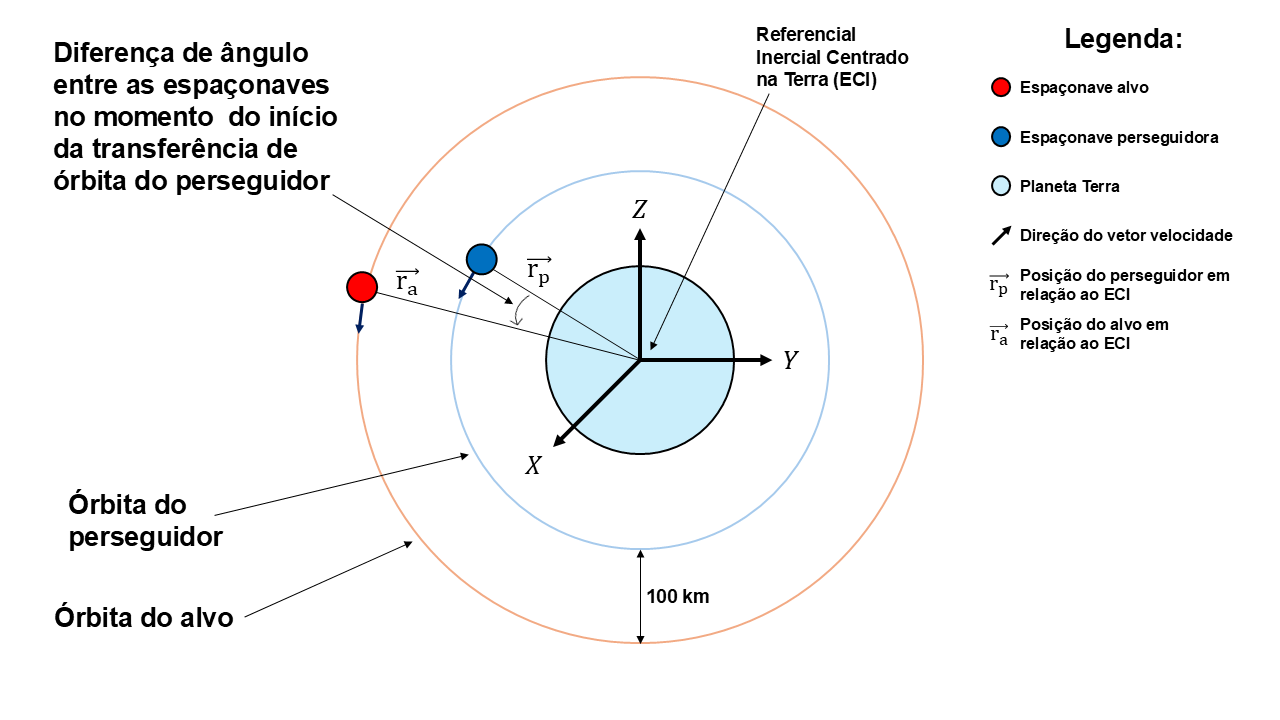
\includegraphics[width=1\linewidth]{2 Revisao bibliografica/Imagens/2 Posicao espaconaves antes da transf de orbita.png}
\caption{Configuração relativa das espaçonaves no início da transferência orbital do perseguidor (sem escala).}
\label{fig_transf_orbita}
\end{figure}

A Figura~\ref{fig_transf_orbita} ilustra a sequência das etapas envolvidas no processo de aproximação.
É apresentada a posição da espaçonave alvo e o movimento relativo realizado pelo perseguidor ao longo das diferentes fases da missão.

\begin{figure}[H]
\centering
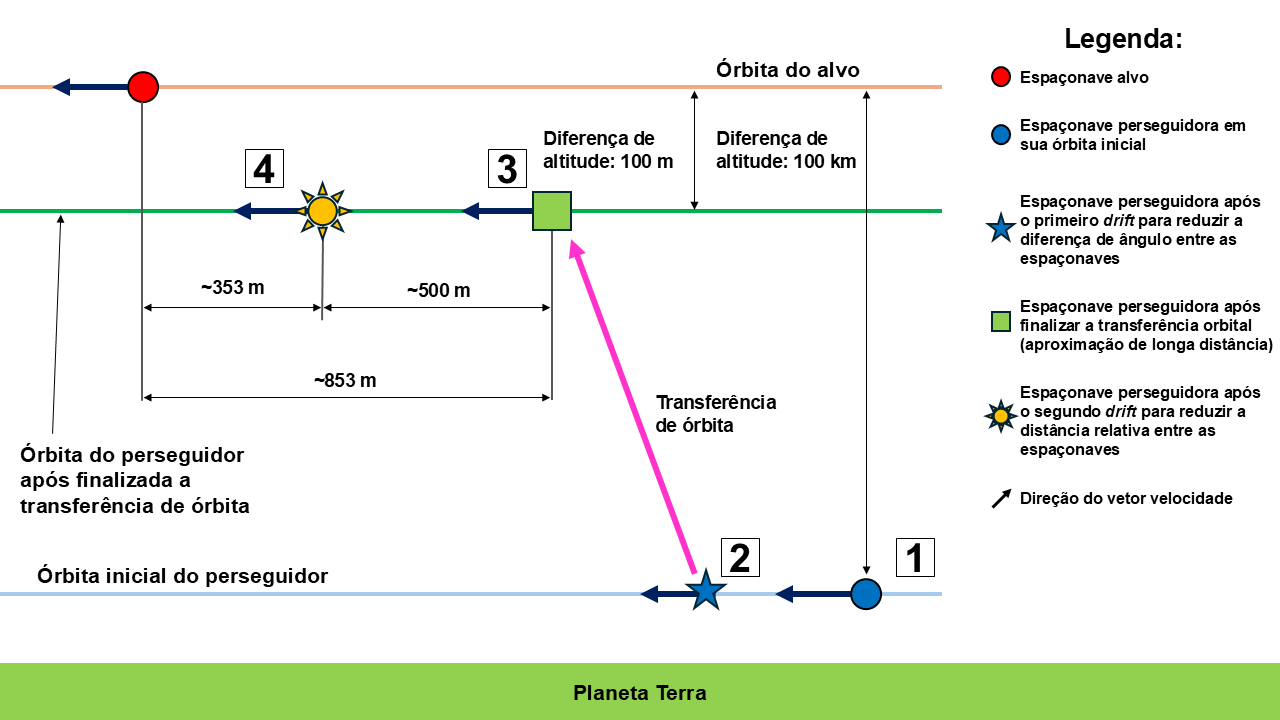
\includegraphics[width=1\linewidth]{2 Revisao bibliografica/Imagens/3 Sequencia das fases.png}
\caption{Sequência das etapas da missão de \gls{rvdb} (sem escala).}
\label{fig_fases_RVDB}
\end{figure}

Os números indicados na Figura~\ref{fig_fases_RVDB} representam as etapas do processo de aproximação, sendo:

\begin{enumerate}
\item após a injeção em sua órbita inicial, o perseguidor realiza uma deriva orbital com o objetivo de reduzir o ângulo de fase em relação ao alvo;
\item execução da manobra de transferência orbital;
\item acomodação do perseguidor na nova órbita e realização de uma nova deriva orbital, enquanto são efetuadas verificações de posição e velocidade relativas;
\item início do movimento relativo no referencial local centrado no alvo.
\end{enumerate}

%%%%%%%%%%%%%%%%%%%%%%

\subsection{Fluxo da aproximação de longa distância}
\label{subsec_fluxo_app_longa_distancia}

O fluxo da etapa de aproximação de longa distância é ilustrado na Figura~\ref{fig_fluxo_app_longa_distancia}. 
Essa fase corresponde ao período inicial da missão em que o perseguidor ainda se encontra a grandes distâncias do alvo, sendo o movimento descrito no referencial inercial. 
Nesse regime, a dinâmica orbital de ambas as espaçonaves é modelada por meio do problema de dois corpos.

\begin{figure}[H]
\centering
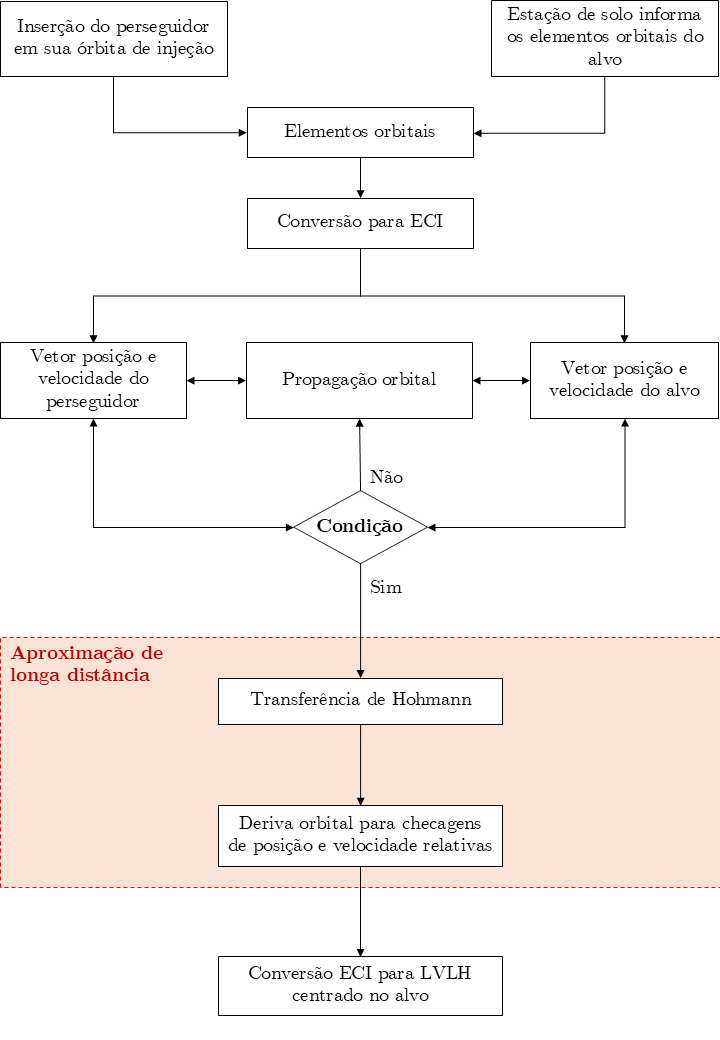
\includegraphics[width=1\linewidth]{3 Procedimento simulacao/Imagens diagrama/2 App longa.png}
\caption{Fluxo da aproximação de longa distância.}
\label{fig_fluxo_app_longa_distancia}
\end{figure}

Inicialmente, são definidos os elementos orbitais do perseguidor e do alvo. 
Os elementos do alvo são assumidos conhecidos e fornecidos pela estação de solo, enquanto os elementos do perseguidor são determinados a partir das condições de injeção orbital. 
A partir desses parâmetros, realiza-se a conversão para o referencial inercial \gls{eci}, obtendo-se os vetores de posição e velocidade de ambas as espaçonaves.

Com os vetores de estado (posição e velocidades no \gls{eci}) definidos, procede-se à propagação orbital das trajetórias do perseguidor e do alvo. 
Durante essa propagação, verifica-se continuamente a condição que determina o momento apropriado para iniciar a manobra de transferência orbital. 
Quando essa condição é satisfeita, é executada uma transferência do tipo Hohmann, cujo objetivo é conduzir o perseguidor a uma órbita com raio inferior ao da órbita do alvo.

Após a execução da transferência, o perseguidor permanece em deriva orbital enquanto são realizadas verificações das condições de posição e velocidade relativas. 
Essa etapa permite avaliar se o alinhamento orbital necessário para o início da aproximação relativa foi atingido. 
Por fim, quando as condições desejadas são satisfeitas, realiza-se a conversão do estado orbital para o referencial \gls{lvlh} centrado no alvo, marcando a transição para a fase de aproximação de curta distância.

